\section{Proposed solution}\label{sec:proposed-solution}
%**************************************************************

TextFooler and BERT-Attack suffer respectively from a lack of context and semantic similarity. 
We tried to combine their strengths in a novel method called SynBA (contextualized Synonym-Based adversarial Attack).
The main idea is to generate a set of synonyms for each word in the sentence, and then select the best synonym for each word based on the context and semantic similarity.

%**************************************************************

\subsection{Intuition}\label{subsec:intuition}

In order to achieve semantic-consistent adversaries, we need to consider the cosine similarity between word embeddings or exploit a synonym dictionary.
While the synonyms retrieved from a thesaurus like WordNet are often somewhat related to the original word, the relationship is often the wrong one for the given context.
Conversely, BERT has the potential to generate more fluent substitutions for an input text.

Our intuition is that the ranked list of candidates for word replacement is obtained from the so called \emph{SynBA score}, a weighted function summing up three scores:
\begin{itemize}
    \item \textbf{MLM score} - the confidence of the candidate obtained by MLM (BERT)
    \item \textbf{Thesaurus score} - a score assigned to synonyms, hyponyms, and hypernyms of the original word in WordNet
    \item \textbf{Word embedding score} - the cosine similarity between the original word and the candidate
\end{itemize}

Combining these three scores, we can obtain a ranked list of candidates that results in a more contextualized and semantically consistent adversary.

%**************************************************************

\subsection{SynBA components}\label{subsec:synba-components}
SynBA has been implemented using TextAttack, a Python framework for implementing adversarial attacks in NLP (refer to section \ref{sec:text-attack} for more details).
Following the framework structure, we decomposed our attack method into four components: a goal function, a set of constraints, a transformation, and a search method.

We reused some of the pre-existing components in TextAttack, such as the \texttt{UntargetedClassification} goal function, the \texttt{GreedyWordSwapWIR} search method and the constraints. 
The innovative part of SynBA is the \texttt{WordSwapMultimodal} transformation, implementing the SynBA score mechanism.
Table \ref{tab:3_3_comparing_components} summarizes the differences between SynBA and the two baselines.

\begin{table}[h]
    \footnotesize
\centering
\begin{tabular}{|c|c|c|c|}
\hline
\textbf{Components} & \textbf{TextFooler} & \textbf{BAE}  & \textbf{SynBA}\\ \hline
Search Method &  Deletion-based &   Deletion-based & Gradient-based\\ 
for Ranking Words & Word Importance & Word Importance & Word Importance \\ \hline
Transformation & Word Embedding & BERT MLM & SynBA score \\ \hline
 & POS  & POS & POS \\ 
 Constraints & USE & USE & Sentence-BERT \\ 
 & Word Embedding Distance &  & Word Embedding Distance \\ 
 &  &  & Max Modification Rate \\ \hline
 
\end{tabular}
\caption{Comparing SynBA components with TextFooler and BAE}
\label{tab:3_3_comparing_components}
\end{table}

%--------------------------------------------------------------
\subsubsection{Search Method}\label{subsubsec:search-method}

The search method is responsible for going through the search space of possible perturbations and finding a sequence of transformations that produce a successful adversarial example.

Greedy algorithms with word importance ranking are linear concerning input length, with a complexity of $\mathcal{O}(W*T)$, where $W$ indicates the number of words in the input, $T$ is the maximum number of transformation options for a given input \cite{journals/corr/abs-2009-06368}. 

So in SynBA we use the \texttt{GreedyWordSwapWIR} search method, which is a greedy search method that iteratively applies the transformation to the input text, and selects the best candidate for each word based on the \acrfull{wir} score.
Words of the given input are ranked according to the importance function. Then, in order of descending importance, each word is substituted with the best candidate given by the transformation
that maximizes the scoring function until the goal is achieved, or all words have been perturbed.

The WIR is gradient-based, which means that it is able to rank the words in the input text exploiting the gradient of the loss function with respect to each token.

It is the same search method used by the attack component in A2T (see section \ref{subsec:a2t}).
Yoo et al. \cite{journals/corr/abs-2009-06368} showed that the gradient-ordering method is the fastest search method and provides a competitive attack success rate when compared to the deletion-based method.
%--------------------------------------------------------------

\subsubsection{Transformation}\label{subsubsec:transformation}

To enforce semantic preservation, we designed the \texttt{WordSwapMultimodal} transformation function, which is not provided by TextAttack.
It computes a set of $k$ perturbations given a word in the input text selected by the search method, where $k$ is the number of candidates to be generated.

The transformation function is based on the SynBA score, which is described in Figure \ref{fig:3_3_synba_score}.
It is calculated for each word in the vocabulary and then they are ranked in descending order.
Tree components are used to compute the SynBA score: the \emph{MLM score}, the \emph{thesaurus score}, and the \emph{word embedding score}.

The \emph{MLM score} is the confidence of the candidate obtained by \texttt{bert-base-uncased}\footnote{\url{https://huggingface.co/bert-base-uncased}} MLM masking the word that we want to perturb.
Since confidence is a probability value, we need to normalize it in order to have each component magnitude in the same range $[0,1]$.
So the vector output of the MLM is rescaled using a min-max scaling:
\begin{equation}
    x^\prime = \frac{x - \min(x)}{\max(x) - \min(x)}
\end{equation}

The \emph{thesaurus score} makes use of WordNet, a lexical database for the English language. Each word in the vocabulary is associated with a score depending on the relation with the original word:
\begin{itemize}
    \item \textbf{synonym} - the score is equal to 1
    \item \textbf{hyponym} - the score is equal to 0.5
    \item \textbf{hypernym} - the score is equal to 0.5
    \item \textbf{antonym} - the score is equal to -100 (to push the antonym out of the top $k$ candidates)
\end{itemize}
If the candidate is not in the WordNet \emph{synset}, the score is equal to 0.

The \emph{word embedding score} is the cosine similarity between the original word and the candidate. We used counter-fitting GloVe vectors \cite{conf/naacl/MrksicSTGRSVWY16} exploiting the property of antonym repeal and synonym attraction. 
This score falls already in the range $[0,1]$, so it does not need to be normalized.

The vocabulary of the MLM is likely different from the one of WordNet and GloVe, so we consider the union of the three vocabularies.
Then the three scores are combined using a weighted sum, where the weights $\lambda_1, \lambda_2, \lambda_3$ are hyperparameters that can be tuned.

Reference words in the original text that are numbers, non-alphabetical, stop words or one-character words are not perturbed, since they could easily influence the meaning of the sentence (e.g. in a movie review, if we alter the number of stars from 5 to 1, the polarity of the review changes).
Meanwhile, candidates that are subwords, punctuations or contain multiple words are discarded.

Before replacing each candidate with the reference word in the input text, we recover the original capitalization of the word, since the MLM and the word embedding models are case insensitive.

\begin{figure}
    \centering
    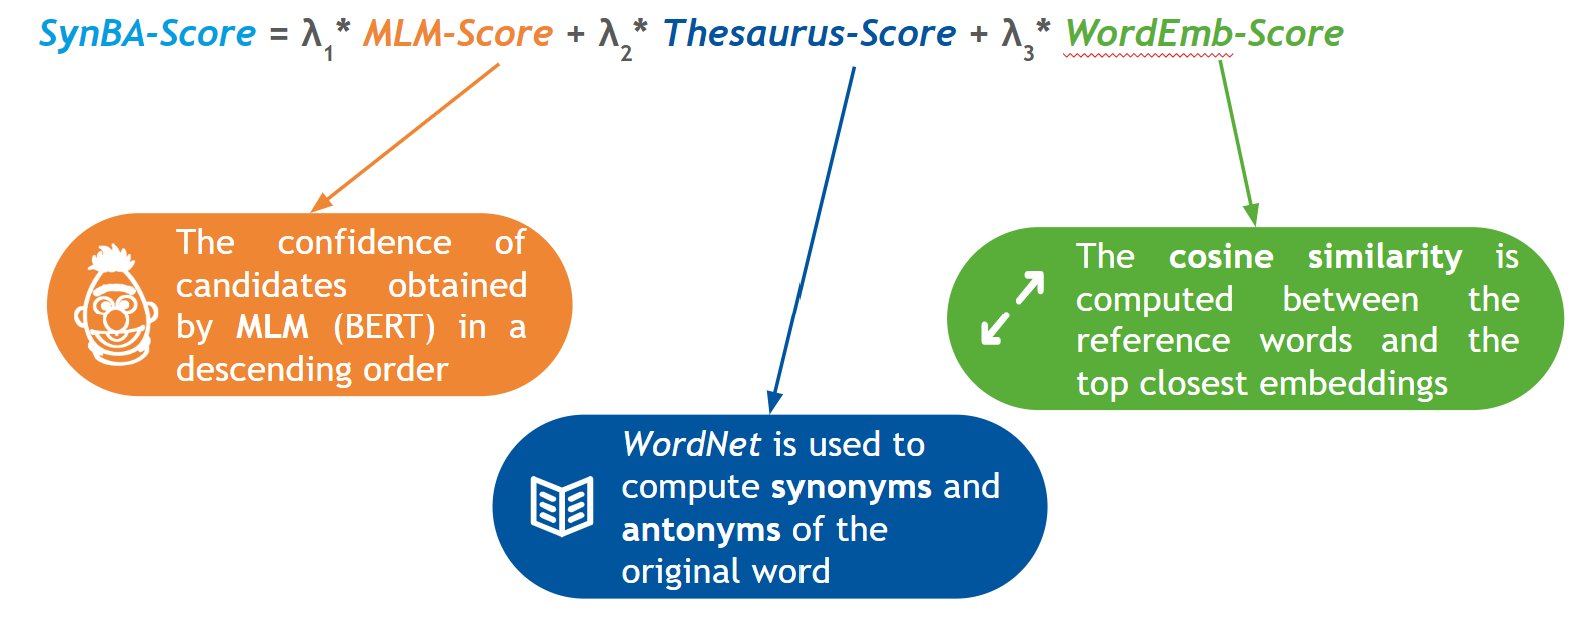
\includegraphics[width=0.8\linewidth]{images/3_3_synba_score.png}
    \caption{SynBA score}
    \label{fig:3_3_synba_score}
\end{figure}

%--------------------------------------------------------------

\subsubsection{Constraints}\label{subsubsec:constraints}

Constraints are used to avoid the generation of adversarial examples that are too different from the original input text.
Those perturbations that do not satisfy all constraints are discarded.

We reused the following constraints, which are already implemented in the framework:
\begin{itemize}
    \item \texttt{PartOfSpeech} - constraints perturbations to only swap words with the same part of speech. It uses the NLTK universal part-of-speech tagger;
    \item \texttt{WordEmbeddingDistance} - throws away perturbations for which the distance between the original word and the candidate is lower than a threshold $t=0.6$;
    \item \texttt{MaxModificationRate} - limits the number of words that can be perturbed in the input text to a maximum percentage $p=0.2\%$. Since text length can vary a lot between samples, and a $p$ modification limit might not make sense for very short text, it is guaranteed that at least 4 words can be perturbed;
    \item \texttt{BERT} - checks whether the \acrfull{sts} between the original and the perturbed text is higher than a threshold $t=0.7$. The  sentence embeddings are computed using a Sentence-BERT \cite{reimers2019sentencebert} pre-trained model. In particular, we used the \texttt{stsb-mpnet-base-v2}\footnote{\url{https://huggingface.co/sentence-transformers/stsb-mpnet-base-v2}} model, which is first trained on NLI data, and then we fine-tuned them on the STS benchmark dataset. This generates sentence embeddings that are especially suitable to measure the semantic similarity between sentence pairs.
    It has a higher STSb performance score ($88.57$) compared to USE ($74.92$). This performance metric is the Spearman rank correlation $\rho$ between the cosine similarity of sentence representations and the gold labels for various STS tasks.
\end{itemize}           
%--------------------------------------------------------------

\subsubsection{Goal Function}\label{subsubsec:goal-function}

The goal function in SynBA is \texttt{UntargetedClassification}, which attempts to minimize the score of the correct label until it is no longer the predicted label.
The attack ends when the predicted label of the perturbed text is different from the original one.
Otherwise, a transformation is performed on the next most important word, until all words are perturbed.

The goal function result status can be:
\begin{itemize}
    \item \texttt{Succeded} - the attack was successful and the predicted label is different from the original one;
    \item \texttt{Failed} - the attack method was not able to find a perturbation that fooled the model;
    \item \texttt{Skipped} - the ground truth label is different from the predicted one
\end{itemize}

%**************************************************************



